\documentclass[border=5pt]{standalone}
\usepackage{tikz}
\usepackage{amsmath}
\usetikzlibrary{arrows.meta}
\begin{document}
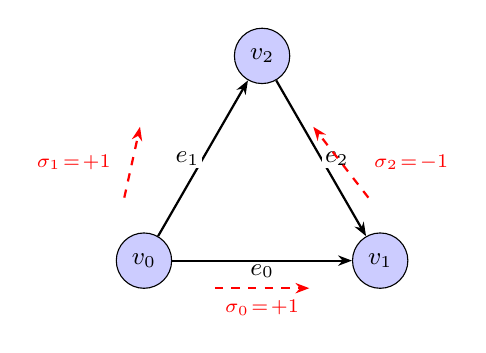
\begin{tikzpicture}[
  vertex/.style={circle, draw, fill=blue!20, minimum size=20pt, inner sep=0pt, font=\small},
  edge label/.style={font=\small, fill=white, inner sep=1pt},
  >={Stealth[length=5pt]}
]
  % Vertices: equilateral triangle, v0 at left, v1 at right, v2 at top
  \node[vertex] (v0) at (0, 0)     {$v_0$};
  \node[vertex] (v1) at (3, 0)     {$v_1$};
  \node[vertex] (v2) at (1.5, 2.6) {$v_2$};

  % Edge e0: v0 -> v1 (bottom)
  \draw[->, thick] (v0) -- node[edge label, below] {$e_0$} (v1);
  % Edge e1: v0 -> v2 (left)
  \draw[->, thick] (v0) -- node[edge label, left]  {$e_1$} (v2);
  % Edge e2: v2 -> v1 (right)
  \draw[->, thick] (v2) -- node[edge label, right] {$e_2$} (v1);

  % Spin arrows (offset from edges, showing sigma = (+1,+1,-1))
  % e0: sigma=+1, same as reference (v0->v1)
  \draw[->, red, thick, dashed] (0.9, -0.35) -- (2.1, -0.35);
  \node[red, font=\scriptsize] at (1.5, -0.6) {$\sigma_0\!=\!+1$};
  % e1: sigma=+1, same as reference (v0->v2)
  \draw[->, red, thick, dashed] (-0.25, 0.8) -- (-0.05, 1.7);
  \node[red, font=\scriptsize, left] at (-0.3, 1.25) {$\sigma_1\!=\!+1$};
  % e2: sigma=-1, opposes reference, so physical flow is v1->v2
  \draw[->, red, thick, dashed] (2.85, 0.8) -- (2.15, 1.7);
  \node[red, font=\scriptsize, right] at (2.8, 1.25) {$\sigma_2\!=\!-1$};
\end{tikzpicture}
\end{document}
